\chapter{Euler's Marvelous Series}

%\vspace*{-15px}

%\begin{figure}[h!]
    %\centering
    %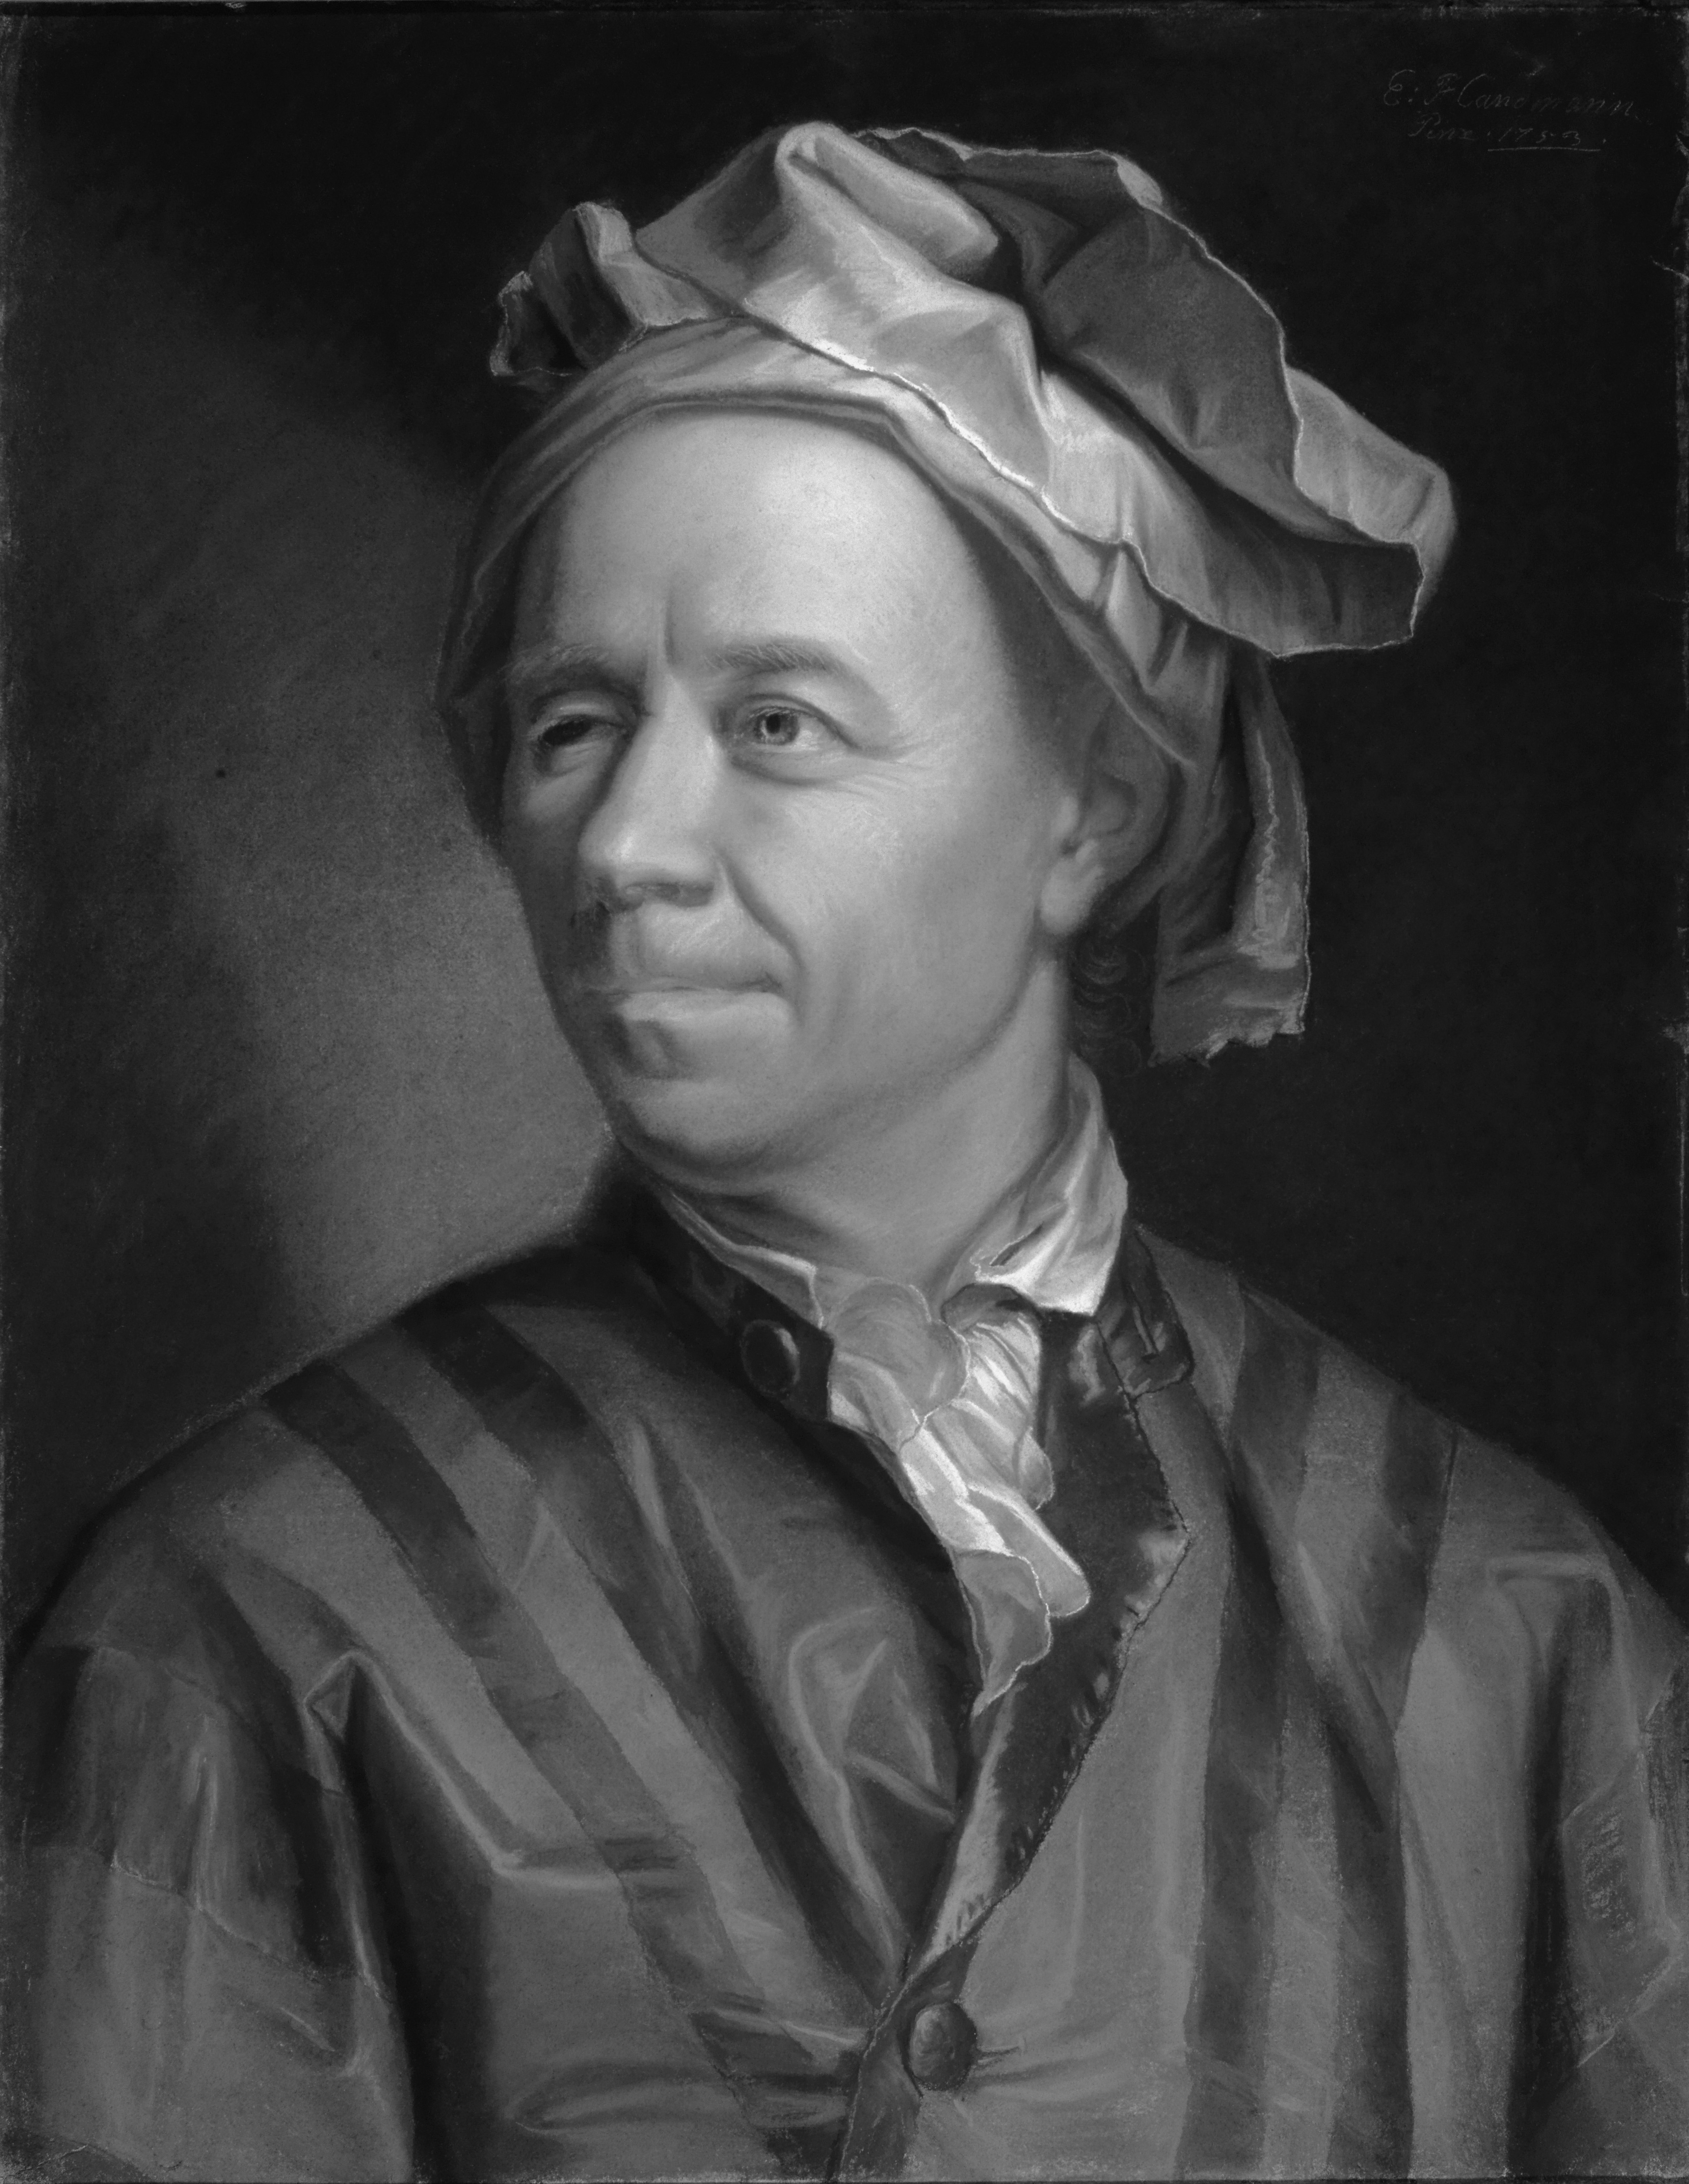
\includegraphics[width=0.4\textwidth]{EulerMarvelousSeries/SummationFormula/photo/Leonhard_Euler_Portrait-modified.jpg}\\
    %Leonhard Euler (1707 - 1783)\label{fig:Euler Portrait}
%\end{figure}

\section{Euler's Summation Formula} \label{sec:summation formula}

The Calculus developed by Sir Isaac Newton (1643 - 1727) and Gottfried Wilhelm Leibniz (1646 - 1716) at the end of the 17th century made the subject of infinite series very popular and useful in mathematics. Before this era, the concept of infinite sums was already encountered in different places in the world. For example, in a treatise written by Archimedes of Syracuse (287 BC - 212 BC) in the 3rd century BC called \textit{Quadrature of the Parabola} \cite{archimedes1897}, there is a visual proof that
$$\frac{1}{4} + \frac{1}{16} + \frac{1}{64} + \frac{1}{256} + \dots = \frac{1}{3}$$
using embedded squares. Next, the decimal representation of numbers, which was introduced in Europe during the 13th century, is simply an application of infinite sums in disguise. For example, the fact that $1/3$ has the decimal expansion $0.333333\dots$ can be reinterpreted as saying that
$$\frac{1}{3} = \frac{3}{10} + \frac{3}{10^2} + \frac{3}{10^3} + \frac{3}{10^4} + \frac{3}{10^5} + \dots$$
In the 14th century, the French mathematician Nicole Oresme (1320 - 1382) showed that the infinite sum 
$$1 + \frac{1}{2} + \frac{1}{3} + \frac{1}{4} + \frac{1}{5} + \dots$$
has an infinite value in the sense that it exceeds any finite quantity. This sum is now called the Harmonic Series. In the same way as Archimedes, Nicole Oresme used a geometric argument to find the following results:
\begin{align*}
    1 + \frac{1}{2} + \frac{1}{4} + \frac{1}{8} + \frac{1}{16} + \dots &= 2 \\
    \frac{1}{2} + \frac{2}{4} + \frac{3}{8} + \frac{4}{16} + \frac{5}{32} + \dots &= 2
\end{align*}
More informations about the work of Nicole Oresme can be found in the article \textit{Mathema-tical Concepts and Proofs from Nicole Oresme} \cite{NicoleOresme}. 

Later, between the 14th and 15th century, members of the Kerala school of astronomy and mathematics, in India, found representations of the sine and the cosine of an angle as an infinite sum. They also found an infinite sum representation of the arctangent of a given quantity. In modern notation, these results can be written as follows:
\begin{align}
    \sin(\theta) &= \theta - \frac{\theta^3}{3!} + \frac{\theta^5}{5!} - \frac{\theta^7}{7!} + \dots \\
    \cos(\theta) &= 1 - \frac{\theta^2}{2!} + \frac{\theta^4}{4!} - \frac{\theta^6}{6!} + \dots \\
    \arctan(x) &= x - \frac{x^3}{3} + \frac{x^5}{5} - \frac{x^7}{7} + \dots \label{Madhava arctan}
\end{align}
These three equations are sometimes called Madhava Series in reference to the Indian mathematician Madhava of Sangamagrama (1340 - 1425), a member of the Kerala school to which these results are attributed. Moreover, by plugging-in $x=1$ in equation (\ref{Madhava arctan}), the following equation is obtained:
\begin{equation} \label{Leibniz / Madhava Series}
    \frac{\pi}{4} = 1 - \frac{1}{3} + \frac{1}{5} - \frac{1}{7} + \frac{1}{9} - \frac{1}{11} + \dots
\end{equation}
This equation was later rediscovered independently by Leibniz which is the reason why people usually call equation (\ref{Leibniz / Madhava Series}) the Leibniz Series. More informations about this result can be found in the article \textit{The Discovery of the Series Formula for $\pi$ by Leibniz, Gregory and Nilakantha} \cite{LeibnizMadhavaSeries}. Compared to the previously discussed results, this one has a particular importance since it involves the constant $\pi$ even though the infinite sum on the right hand side doesn't seem more complicated than the ones discussed above. This result is a first hint that some seemingly simple infinite sums can have unexpected behaviors.

Finally, in 1650, the Italian mathematician Pietro Mengoli (1626 - 1686) publishes his book \textit{Novæ quadraturæ arithmeticæ, seu de additione fractionum} \cite{mengoli1650nouæ} in which he proves various results about infinite sums. For example, he proves that the Harmonic Series is infinite, and also finds the values of
$$\frac{1}{1\cdot(1 + r)} + \frac{1}{2\cdot(2 + r)} + \frac{1}{3\cdot(3 + r)} + \frac{1}{4\cdot(4 + r)} + \dots$$
where $r$ is any integer between 1 and 10. However, he was unable to find the value to which the series
$$\frac{1}{1^2} + \frac{1}{2^2} + \frac{1}{3^2} + \frac{1}{4^2} + \dots$$
converges to (which is the case $r=0$ of the previous sums). Thus, we see through these examples that before the works of Newton and Leibniz, infinite sums already made their appearance in various contexts in time.

Even though some specific examples of infinite sums were already studied in the previous centuries, they really became central in  mathematics when the tools of calculus became available. For example, with his method of fluxions, Newton rediscovered the Madhava Series for the sine and cosine functions and was able to solve differential equations. The tools of calculus gave the perfect framework for what is begining to be called series or infinite series.

Later in that period, in 1689, the Swiss mathematician Jakob Bernoulli (1655 - 1705) wrote his \textit{Tractatus de seriebus infinitis}, a treatise on infinite series in which he discusses the limiting values of various series such as geometric series, telescoping series, the harmonic series and other types of series. For example, he derives the following formula for geometric series:
\begin{equation}
    a + ar + ar^2 + ar^3 + \dots = \frac{a}{1-r}, \qquad \quad -1 < r < 1.
\end{equation}
He also studied some more specific examples such as
\begin{equation}\label{telescoping series}
    \begin{split}
        & 1 + \frac{1}{3} + \frac{1}{6} + \frac{1}{10} + \frac{1}{15} + \frac{1}{21} + \frac{1}{28} + \dots \\
        & = \frac{2}{1(1+1)} + \frac{2}{2(2+1)} + \frac{2}{3(3+1)} + \frac{2}{4(4+1)} + \dots = 2
    \end{split}
\end{equation}
using the fact that it is a telescoping series. As his predecessors, he gave a new proof of the divergence of the Harmonic Series. Finally, when considering the series of the reciprocals of the squares 
$$\frac{1}{1^2} + \frac{1}{2^2} + \frac{1}{3^2} + \frac{1}{4^2} + \dots,$$
he was able to show that it must have a finite limiting value, i.e., that the series converges, by using the inequality 
$$\frac{1}{n^2} \leq \frac{2}{n(n+1)}$$
and combining it with equation (\ref{telescoping series}) to obtain
$$1 + \frac{1}{4} + \frac{1}{9} + \frac{1}{16} + \dots \leq 1 + \frac{1}{3} + \frac{1}{6} + \frac{1}{10} + \dots = 2 < \infty.$$
However, he was unable to find the precise value to which the series converges to and wrote in his \textit{Tractatus} that "great will be our gratitude" if anyone finds and communicates this limiting value. This became known as the Basel Problem (since the mathematician wrote from Basel in Switzerland) and it remained unsolved for decades.

Notice that this series converges very slowly since the individual terms don't approach zero fast enough. This makes the problem even harder since a good strategy for finding the value of a series is to find the sum of the first 20 terms (for example) and guess the limit of the series from this approximation. However, with the series of the reciprocals of the squares, taking the sum of the first 200 terms gives an approximation which is only correct for one decimal.

The first mathematician to make some significant progress on the Basel Problem is a young Swiss mathematician who would soon become the most prolific mathematician of all time. This mathematician is obviously the great Leonhard Euler. 

\subsection*{Enter Euler}

Born in the town of Basel on the 15th of April in 1707, Leonhard Euler is the son of the pastor Paul Euler. From a young age, Leonhard received schooling in mathematics from different persons. First, from his father who had taken courses in mathematics from Jakob Bernoulli at the University of Basel. Then, when attending the University of Basel in 1720 at the age of 13, from Johann Bernoulli (1667 - 1748), Jakob Bernoulli's younger brother. Johann Bernoulli had a great influence on Euler for three reasons, he was one of the top mathematician of his time, they met every saturday afternoon to discuss about mathematics, and because he helped Euler get his father's consent to become a mathematician instead of a pastor. In 1727, Euler joined Daniel Bernoulli, Johann Bernoulli's son, to take a position in the department of mathematics at the Imperial Russian Academy of Sciences in Saint Petersburg. It is here that most of the papers presented in this chapter will be written.

Euler's first contribution to the Basel Problem can be found in his article \textit{De summatione innumerabilium progressionum} \cite{eulerE20}, written in 1731 and published in 1738. In this article, using many integral tricks and algebraic manipulations, Euler was able to obtain the formula
\begin{equation} \label{zeta 2 and (ln 2)^2}
    \frac{1}{1^2} + \frac{1}{2^2} + \frac{1}{3^2} + \dots = \left(\frac{1}{2^0\cdot 1^2} + \frac{1}{2^1\cdot 2^2} + \frac{1}{2^2\cdot 3^2} + \frac{1}{2^3\cdot 4^2} + \dots \right) + (\ln 2)^2
\end{equation}
which relates the series of the reciprocals of the squares to a series which converges much faster to which is added a constant term that can be computed very precisely. With only 20 terms of the right hand side series, Euler is able to obtain the following approximation:
$$1 + \frac{1}{4} + \frac{1}{9} + \frac{1}{16} + \frac{1}{25} + \dots = 1.644934$$
He notices himself that such an approximation can only be obtained by adding more than a thousand terms of the series on the left hand side. Using computers, it turns out that such an approximation would require to sum more than 15 millions terms of the original series, which makes this result already very remarkable. Again, this shows how slowly the original series converges.

Three years later, in the article \textit{Methodus universalis serierum convergentium sum-mas quam proxime inveniendi} \cite{eulerE46} written in June 1735 and published in 1741, Euler found another way of approximating the sum of the reciprocals of the squares. He presented a general geometric method for approximating series using integrals. At the end of the paper, he applied his method to the series of the reciprocals of the square. He considered \autoref{fig:visual sum vs integral}
\begin{figure}[h!] 
    \centering
      \begin{tikzpicture}[scale=0.7]
        \begin{axis}[
            axis lines = left,
            xmin=0.5,
            ymin=0,
            ymax=1.3,
            ymajorticks=false
        ]
    
        \addplot [domain=1:5.3, samples=100, color=black, name path=y] {(1/x^2) + 0.001} node[above=1cm, pos=0.5] {$\displaystyle y = \frac{1}{x^2}$};

        \addplot [domain=1:5,samples=2, color=black, name path=g,]{0};
        \addplot[blue, opacity=0.4] fill between[of=g and y, soft clip={domain=1:5}];
    
        \addplot [domain=1:2,samples=2, color=red, opacity=0.4, name path=f1,]{1};
        \addplot[red, opacity=0.4] fill between[of=f1 and y, soft clip={domain=1:2}];
    
        \addplot [domain=2:3,samples=2, color=red, opacity=0.4, name path=f2,]{0.251};
        \addplot[red, opacity=0.4] fill between[of=f2 and y, soft clip={domain=2:3}];
    
        \addplot [domain=3:4,samples=2, color=red, opacity=0.4, name path=f3,]{0.1121};
        \addplot[red, opacity=0.4] fill between[of=f3 and y, soft clip={domain=3:4}];
        
        \addplot [domain=4:5,samples=2, color=red, opacity=0.4, name path=f4,]{0.0635};
        \addplot[red, opacity=0.4] fill between[of=f4 and y, soft clip={domain=4:5}];

        \end{axis}
    \end{tikzpicture}
    \caption{Visual interpretation of}
    \text{$1 + \frac{1}{2^2} + \frac{1}{3^2} + \frac{1}{4^2} + \dots$}
    \label{fig:visual sum vs integral}
\end{figure}
in which the blue and red area represents the value of the sum of the reciprocals of the squares. We can see that this sum is greater than the blue area under the curve $y = \frac{1}{x^2}$ between $x=1$ and $x = \infty$. But Euler's goal was to approximate the red area above the curve. Using some calculus and geometry, he was able to derive the following approximation of the total shaded area:
$$1 + \frac{1}{4} + \frac{1}{9} + \frac{1}{16} + \frac{1}{25} + \dots = 1.644920$$
which is only true for the first four decimals. It seems like this method is worst than the previous one since it only gives an approximation true for the first four decimals. However, Euler was on track to develop a new very powerful method.

\subsection*{The Summation Formula}

As for the previous method, Euler's goal was to approximate the difference between a series and the integral of the general term of the series. In his paper \textit{Methodus generalis summandi progressiones} \cite{eulerE25}, written in 1732 and published in 1738, Euler mentions without proof such a formula that links a series to its corresponding integral. He then wrote another article called \textit{Inventio summae cuiusque seriei ex dato termino generali} \cite{eulerE47}, written in October 1735 and published in 1741, to go over the proof of his formula and apply it to approximate some series. Let's dive into this last paper to understand his formula. 

The paper starts with an important preliminary result. Take a function $y$ which can be expanded as follows:
$$y(x) = a_0 + a_1x + a_2x^2 + a_3x^3 + a_4x^4 + \dots,$$
then for any $\alpha$ and by the Binomial Theorem:
\begin{align*}
    y(x+\alpha) &= \ a_0 \\
    &+ \left(a_1 x \ \, \, \! + a_1 \alpha\right) \\
    &+ \left(a_2 x^2 + 2a_2 x \alpha \ \ \!+ a_2 \alpha^2\right) \\
    &+ \left(a_3 x^3 + 3a_3 x^2 \alpha + 3 a_3 x\alpha^2 \, \, \,  + a_3 \alpha^3\right) \\
    &+ \left(a_4 x^4 + 4a_4 x^3 \alpha + 6 a_4 x^2 \alpha^2 + 4 a_4 x \alpha^3 + a_4 \alpha^4 \right) \\
    &+ \dots
\end{align*}
Now, if we sum the right hand sum column by column, we obtain
\begin{align*}
    y(x+\alpha) &= (a_0 + a_1 x + a_2 x^2 + a_3 x^3 + a_4 x^4 + \dots) \\
    &+ \frac{\alpha}{1}(a_1 + 2a_2x + 3a_3 x^2 + 4 a_4 x^3 + \dots) \\
    &+ \frac{\alpha^2}{1\cdot 2}(2a_2 + 3\cdot 2 a_3x + 4\cdot 3 a_4 x^2 + \dots) \\
    &+ \frac{\alpha^3}{1\cdot 2 \cdot 3}(3\cdot 2 a_3 + 4\cdot 3 \cdot 2 a_4 x + \dots)\\
    &+ \dots
\end{align*}
Finally, we can recognize that the expressions inside the prentheses are simply the successive derivatives of $y$. It follows that 
\begin{equation} \label{Taylor's Formula}
    y(x + \alpha) = y(x) + \frac{\alpha dy}{1\cdot dx} + \frac{\alpha^2d^2y}{1\cdot 2\cdot dx^2} + \frac{\alpha^3d^3y}{1\cdot 2\cdot 3 \cdot  dx^3} + \frac{\alpha^4d^4y}{1\cdot 2\cdot 3 \cdot 4\cdot dx^4} + \dots
\end{equation}
Euler attributes this result to the mathematician Brook Taylor (1685 - 1731) who is now known for his work on Taylor Series. After obtaining this formula, Euler introduced the main problem of the article. Suppose we are given a function $f(x)$ and we define the new function
\begin{equation}
    S(x) = f(1) + f(2) + f(3) + \dots + f(x),
\end{equation} 
How can we find a simpler expression of the function $S(x)$ ? For example, if $f(x) = x$, then $S(x)$ is simply $x(x+1)/2$. First, he noticed that by definition of $S(x)$, we have
$$S(x - 1) = S(x) - f(x)$$
and so
\begin{equation} \label{f = difference of S}
    f(x) = S(x) - S(x-1).
\end{equation}
Moreover, using equation (\ref{Taylor's Formula}) with $y = S$ and $\alpha = -1$, he obtained
$$S(x-1) = S(x) - \frac{dS}{1\cdot dx} + \frac{d^2S}{1\cdot 2\cdot dx^2} - \frac{d^3S}{1\cdot 2\cdot 3 \cdot  dx^3} + \frac{d^4S}{1\cdot 2\cdot 3 \cdot 4\cdot dx^4} + \dots$$
Even if $S(x)$ was defined for positive integers only, Euler assumed that it could be treated as an infinitely differentiable function. This can be explained by the fact that our goal is to find a nice function that interpolates the partial sums of $f(x)$. Hence, we are not defining $S(x)$ as the partial sums of $f(x)$, instead, we are trying to deduce the formula of such a function $S(x)$ if it exists. After this last equation, he substituted it into equation (\ref{f = difference of S}) to get
\begin{equation} \label{f in terms of S}
    f(x) = \frac{dS}{1\cdot dx} - \frac{d^2S}{1\cdot 2\cdot dx^2} + \frac{d^3S}{1\cdot 2\cdot 3 \cdot  dx^3} - \frac{d^4S}{1\cdot 2\cdot 3 \cdot 4\cdot dx^4} + \dots
\end{equation}
However, Euler notices that the goal is to find a new expression of $S(x)$, not of $f(x)$. The last equation expresses $f(x)$ in terms of $S'(x)$ and its derivatives. Hence, his next step is to invert this equation, i.e., to write $S'(x)$ in terms of $f(x)$ and its derivatives. To do so, he assumes that
\begin{equation} \label{S' undeterminate coef}
\frac{dS}{dx} = \alpha_0 f(x) + \alpha_1 \frac{df}{dx} + \alpha_2 \frac{d^2f}{dx^2} + \alpha_3 \frac{d^3f}{dx^3} + \alpha_4 \frac{d^4f}{dx^4} + \dots
\end{equation}
and so now the goal is to find the coefficients $\alpha_0, \alpha_1, \alpha_2, \alpha_3, \alpha_4, \dots$. To determine these coefficients, Euler differentiated both sides of equation (\ref{S' undeterminate coef}) to obtain:
\begin{align*}
    \frac{dS}{dx} &= \alpha_0 f(x) + \alpha_1 \frac{df}{dx} + \alpha_2 \frac{d^2f}{dx^2} + \alpha_3 \frac{d^3f}{dx^3} + \alpha_4 \frac{d^4f}{dx^4} + \dots\\
    \frac{d^2S}{dx^2} &= \alpha_0 \frac{df}{dx} + \alpha_1 \frac{d^2f}{dx^2} + \alpha_2 \frac{d^3f}{dx^3} + \alpha_3 \frac{d^4f}{dx^4} + \dots\\
    \frac{d^3S}{dx^3} &= \alpha_0 \frac{d^2f}{dx^2} + \alpha_1 \frac{d^3f}{dx^3} + \alpha_2 \frac{d^4f}{dx^4} + \dots\\
    \frac{d^4S}{dx^4} &= \alpha_0 \frac{d^3f}{dx^3} + \alpha_1 \frac{d^4f}{dx^4} + \dots\\
    \frac{d^5S}{dx^5} &= \alpha_0 \frac{d^4f}{dx^4} + \dots\\
\end{align*}
He then substituted these equations into equation (\ref{f in terms of S}) to get:
\begin{align*}
    f(x) &= \frac{1}{1}\left(\alpha_0 f(x) + \alpha_1 \frac{df}{dx} + \alpha_2 \frac{d^2f}{dx^2} + \alpha_3 \frac{d^3f}{dx^3} + \alpha_4 \frac{d^4f}{dx^4} + \dots\right) \\
    &-\frac{1}{2}\left(\alpha_0 \frac{df}{dx} + \alpha_1 \frac{d^2f}{dx^2} + \alpha_2 \frac{d^3f}{dx^3} + \alpha_3 \frac{d^4f}{dx^4} + \dots\right) \\
    &+ \frac{1}{6}\left(\alpha_0 \frac{d^2f}{dx^2} + \alpha_1 \frac{d^3f}{dx^3} + \alpha_2 \frac{d^4f}{dx^4} + \dots\right) \\
    &- \frac{1}{24}\left(\alpha_0 \frac{d^3f}{dx^3} + \alpha_1 \frac{d^4f}{dx^4} + \dots\right) \\
    &+ \frac{1}{120}\left(\alpha_0 \frac{d^4f}{dx^4} + \dots\right) \\
    &- \dots
\end{align*}
Next, by expanding the right hand side and grouping the terms by their respective derivatives of $f(x)$, Euler obtained the following equation:
\begin{align*}
    f(x) &= \alpha_0 f(x) \\
    &+ \left(\alpha_1 - \frac{\alpha_0}{2}\right)\frac{df}{dx} \\
    &+ \left(\alpha_2 - \frac{\alpha_1}{2} + \frac{\alpha_0}{6} \right)\frac{d^2f}{dx^2}  \\
    &+ \left(\alpha_3 - \frac{\alpha_2}{2} + \frac{\alpha_1}{6} - \frac{\alpha_0}{24}\right)\frac{d^3f}{dx^3} \\
    &+ \left(\alpha_4 - \frac{\alpha_3}{2} + \frac{\alpha_2}{6} - \frac{\alpha_1}{24} + \frac{\alpha_0}{120}\right)\frac{d^4f}{dx^4} \\
    &+ \dots 
\end{align*}
Finally, Euler deduced from this equation that $\alpha_0$ must be 1 and that all the other coefficients in front of the derivatives of $f'(x)$ must be zero. It follows that
\begin{align*}
    \alpha_0 &= 1 \\
    \alpha_1 &= \frac{\alpha_0}{2} \\
    \alpha_2 &= \frac{\alpha_1}{2} - \frac{\alpha_0}{6} \\
    \alpha_3 &= \frac{\alpha_2}{2} - \frac{\alpha_1}{6} + \frac{\alpha_0}{24} \\
    \alpha_4 &= \frac{\alpha_3}{2} - \frac{\alpha_2}{6} + \frac{\alpha_1}{24} - \frac{\alpha_0}{120} \\
    & etc \dots
\end{align*}
which implies that each $\alpha_n$ can be determined by its predecessors. Euler used these formulas to compute the first $\alpha_n$'s:
$$\alpha_0 = 1 \qquad \alpha_1 = \frac{1}{2} \qquad \alpha_2 = \frac{1}{12} \qquad \alpha_3 = 0 \qquad \alpha_4 = - \frac{1}{720} \qquad \alpha_5 = 0 \qquad \alpha_6 = \frac{1}{30240}$$
from which he finally obtained
\begin{equation}
    S'(x) = f(x) + \frac{df}{2\cdot dx} + \frac{d^2f}{12\cdot dx^2} - \frac{d^4f}{720\cdot dx^4} + \frac{d^6f}{30240\cdot dx^6} - \dots
\end{equation}
Therefore, the last step is simply to integrate this equation to obtain a new expression for $S(x)$:
\begin{equation}\label{Euler Summation Formula 1}
    \boxed{S(x) = \int f(x)dx + \frac{f(x)}{2} + \frac{df}{12\cdot dx} - \frac{d^3f}{720\cdot dx^3} + \frac{d^5f}{30240\cdot dx^5} - \dots + C}
\end{equation}
where $C$ is the constant of integration that makes $S(0) = 0$, and where the coefficient in front of the $n$th derivative of $f(x)$ is $\alpha_{n+1}$. From the condition that $S(0) = 0$ we have that our integration constant is
\begin{equation}
    C = -\left[\int f(x)dx + \frac{f(x)}{2} + \frac{df}{12\cdot dx} - \frac{d^3f}{720\cdot dx^3} + \frac{d^5f}{30240\cdot dx^5} - \dots\right]_{x = 0}
\end{equation}
since adding this constant on the right hand side of equation (\ref{Euler Summation Formula 1}) and evaluating the expression on the right at $x = 0$ would give $S(0) = 0$. 

This is the now famous Euler Summation Formula. There is a lot to say about this derivation. First, we can clearly see how low were the standards in terms of rigor at that time. Such a proof would never be accepted today. However, since Euler, other proofs were provided for this formula so we can rest our mind and be sure of its validity. The usefulness of this formula may not be obvious for the moment since it seems like Euler have made the problem harder. Our first expression for $S(x)$ was a simple finite sum involving no derivatives. This new expression of $S(x)$ is an infinite sum involving derivatives of $f(x)$ of arbitrarily high orders. At least it is clear now that $S(x)$ is defined over way more numbers than just the positive integers, and that it is differentiable. But to really understand how powerful this formula is, let's see it in action.

\subsection*{The Formula in Action}

For his first example, Euler took the function $f(x) = x$. Notice that with this function, the constant $C$ is simply equal to $-1/12$ since the only non-zero term in the formula for $C$ is the one involving the first derivative of $f(x)$. Thus, we get
$$S(x) = \int xdx + \frac{x}{2} + \frac{1}{12} - 0 + 0 - \dots +C= \frac{x(x+1)}{2}$$
which is indeed the correct formula. Similarly, with $f(x) = x^2$, he obtained
$$S(x) = \frac{x^3}{3} + \frac{x^2 }{2} + \frac{x}{6} = \frac{x(x+1)(2x+1)}{6}$$
which is, again, the correct formula. Since taking the successive derivatives of the function $f(x) = x^m$ is an easy task, we can see how Euler's formula can be used to recover all the formulas for the sum of the first $n$ powers of $m$. And this is exactly what Euler did, from his formula, he deduced the formula for the specific case $f(x) = x^m$ and from that, he deduced the equivalent of the two previous equations (which were the case $m=1$ and $m=2$) for the cases $m=3, 4, 5, ..., 15, 16$. In \autoref{fig:Extract Euler}, the symbole $\int x^m$ denotes the sum $1^m + 2^m + 3^m + \dots + x^m$.

\begin{figure}[h]
    \centering
    \includegraphics[width=0.7\textwidth]{EulerMarvelousSeries/SummationFormula/photo/Capture d’écran, le 2025-06-20 à 11.39.28.png}
    \caption{Extract from Euler's paper}
    \label{fig:Extract Euler}
\end{figure}

After these examples, Euler finished his paper by returning on the original problem of approximating the sum of the reciprocals of the squares. Euler let $f(x) = \frac{1}{x^2}$ and noticed that he could not apply the formula directly since computing the constant $C$ would require dividing by $0$. Hence, Euler split the sum as follows:
$$1 + \frac{1}{4} + \frac{1}{9} + \frac{1}{16} + \frac{1}{25} + \dots = \left(1 + \frac{1}{4} + \dots + \frac{1}{100}\right) + \left(\frac{1}{121} + \frac{1}{144} + \frac{1}{169} + \dots\right)$$
He computed by hand the first ten terms of the series to get
\begin{equation} \label{Approximation for first ten terms}
    1 + \frac{1}{4} + \dots + \frac{1}{81} + \frac{1}{100} = 1.549767731166540
\end{equation}
and then used his summation formula to approximate the remaining terms:
\begin{equation}
    S(x) = \frac{1}{11^2} + \frac{1}{12^2} + \frac{1}{13^2} + \dots + \frac{1}{x^2}.
\end{equation}
In the previous equation, the initial condition now becomes $S(10) = 0$ instead of $S(0) = 0$ because the first term has index $x = 11$. Therefore, the constant term is
\begin{equation} \label{C for S(10)=0}
    C = -\int f(x)dx\bigg\rvert_{x=10} - \frac{f(x)}{2}\bigg\rvert_{x=10} - \frac{df}{12\cdot dx}\bigg\rvert_{x=10} + \frac{d^3f}{720\cdot dx^3}\bigg\rvert_{x=10} - \frac{d^5f}{30240\cdot dx^5}\bigg\rvert_{x=10} + \dots
\end{equation}
Euler then computed the first successive derivatives of $f(x)$ to obtain
$$\int f(x)dx = -\frac{1}{x} \qquad  \frac{df}{dx} = -\frac{2}{x^3} \qquad \frac{d^3f}{dx^3} = -\frac{2\cdot 3 \cdot 4}{x^5} \qquad \frac{d^5f}{dx^5} = -\frac{2\cdot 3 \cdot 4 \cdot 5 \cdot 6}{x^7}$$
and so plugging this into equation (\ref{C for S(10)=0}) gives
$$C = \frac{1}{10} - \frac{1}{200} + \frac{1}{6000} - \frac{1}{3000000} + \frac{1}{420000000} - \frac{1}{30000000000} + \dots$$
which converges really fast, and hence, can be approximated really well. Therefore, using his summation formula, he obtained 
\begin{equation} \label{Approximation other terms}
    \frac{1}{11^2} + \frac{1}{12^2} + \dots + \frac{1}{x^2} = \left(-\frac{1}{x} + \frac{1}{2x^2} - \frac{1}{6x^3} + \frac{1}{30x^5} - \dots\right) + C
\end{equation}
He then combined equations (\ref{Approximation for first ten terms}) and (\ref{Approximation other terms}) to get
$$1 + \frac{1}{4} + \dots + \frac{1}{x^2} = 1.549767731166540 + C + \left(-\frac{1}{x} + \frac{1}{2x^2} - \frac{1}{6x^3} + \frac{1}{30x^5} - \dots\right)$$
Finally, letting $x$ go to infinity gives
\begin{equation} \label{approximation zeta 2}
    \boxed{1 + \frac{1}{4} + \frac{1}{9} + \frac{1}{16} + \dots = 1.64493406684822643647}
\end{equation}
which is an apprixomation with twenty correct decimals! It was mentioned earlier in this section that to obtain an approximation correct to six decimals, it would require taking the sum of more than the first 15 million terms of the original series. Similarly, to get an approximation with 20 correct decimals, it is required to sum more than the first $10^{20}$ terms of the original series. The last two examples he provided in his paper are similar approximations of the sum of the inverse of the cubes and the sum of the inverse of the biquadrates:
\begin{align}
    1 + \frac{1}{8} + \frac{1}{27} + \frac{1}{64} + \dots &= 1.202056903159594 \\
    1 + \frac{1}{16} + \frac{1}{81} + \frac{1}{256} + \dots &= 1.0823232337110824
\end{align}

With this single summation formula and its countless applications, Euler clearly stands as one of the most ingenious mathematician of his time. However, you may guess that this is only the begining. Euler went further than that. It turns out that only two months after writting his paper \textit{Inventio summae...} which we just presented, Euler solved the Basel Problem. Not only he recognized the exact value of the number he approximated in equation (\ref{approximation zeta 2}), but he also found a way to prove it. The next section will be focused on Euler's paper which contains his solution to the Basel Problem. 

The Euler Summation Formula which was introduced in this section will also appear in the next sections. Euler used it a lot throughout his mathematical career because it turns out that there is still a lot to say about this formula, especially concerning the coefficients $\alpha_0, \alpha_1, \alpha_2, \dots$ which will have a great importance later. \\

\noindent {\Large\textbf{Exercises}}

\begin{exercise}
    In this exercise, the sequence $H_n = \sum_{k=1}^{n}\frac{1}{k}$ denotes the sequence of partial sums of the Harmonic Series. In the article \textit{De summatione innumerabilium progressionum} written in 1731, Euler interpolated the sequence $H_n$ using the function
    $$H(x) = \int_{0}^{1}\frac{1-t^x}{1-t}dt.$$
    \begin{enumerate}[label=(\alph*)]
        \item Prove that $H(n) = H_n$ for all $n \geq 1$.
        \item Find the value of $H(1/2)$.
        \item Prove that $H(x + 1) = H(x) + \frac{1}{x+1}$ for all $x > 0$.
        \item Deduce a general formula for $H(n + \frac{1}{2})$. 
    \end{enumerate}
\end{exercise}

\begin{exercise}
    In the same paper as the one mentioned in the previous exercise, Euler proves that 
    $$\frac{1}{1^2} + \frac{1}{2^2} + \frac{1}{3^2} + \frac{1}{4^2} + \dots = \left(\frac{1}{2^0\cdot 1^2} + \frac{1}{2^1\cdot 2^2} + \frac{1}{2^2\cdot 3^2} + \frac{1}{2^3\cdot 4^2} + \dots \right) + (\ln 2)^2$$
    as a corollary of a more general method. To make Euler's proof easier to understand, this exercise outlines Euler's argument applied to the specific case of the sum of the reciprocals of the squares. This version of Euler's proof comes from the article \textit{Euler and the Zeta Function} written by Raymond Ayoub.
    \begin{enumerate}[label=(\alph*)]
        \item Show that
        $$-\frac{\ln(1-x)}{x} = 1 + \frac{x}{2} + \frac{x^2}{3} + \frac{x^3}{4} + \frac{x^4}{5} + \dots$$
        \item Deduce the following new expression of the sum of the reciprocals of the squares
        $$1 + \frac{1}{4} + \frac{1}{9} + \frac{1}{25} + \dots = -\int_{0}^{1}\frac{\ln(1-x)}{x}dx.$$
        \item Split the integral on right hand side at $x= \frac{1}{2}$ and define
        $$I_1 = -\int_{0}^{\frac{1}{2}}\frac{\ln(1-x)}{x}dx \qquad \qquad I_2 = -\int_{\frac{1}{2}}^{1}\frac{\ln(1-x)}{x}dx.$$
        so that the sum of the reciprocals of the squares is equal to $I_1 + I_2$. Use part (a) to find
        $$I_1 = \frac{1}{2^1\cdot 1^2} + \frac{1}{2^2\cdot 2^2} + \frac{1}{2^3\cdot 3^2} + \frac{1}{2^4\cdot 4^2} + \dots$$
        \item In the integral $I_2$, make the change of variable $u = 1-x$ and expand the resulting denominator in a power series. From this, make an integration by parts term-by-term to obtain
        $$I_2 = I_1 + (\ln 2)^2.$$
        \item Deduce the desired formula from part (c) and part (d).
    \end{enumerate}
\end{exercise}

\begin{exercise}
    Use Taylor's Formula (equation (\ref{Taylor's Formula})) to derive the following identities:
    \begin{enumerate}[label=(\alph*)]
        \item $e^{a+b} = e^ae^b$
        \item $\sin(a+b) = \sin(a)\cos(b) + \cos(a)\sin(b)$
        \item $\cos(a+b) = \cos(a)\cos(b) - \sin(a)\sin(b)$
    \end{enumerate}
\end{exercise}

\begin{exercise}
    Use Euler's Summation Formula (equation (\ref{Euler Summation Formula 1})) to find the formula for the sum of the first $n$ cubes. By induction, prove that your formula is correct for all positive integers.
\end{exercise}

\begin{exercise}
    Use Euler's Summation Formula (equation (\ref{Euler Summation Formula 1})) to find the general formula for the sum of the $n$ first powers of $m$.
\end{exercise}

\begin{exercise} \label{Exercise on Euler-Mascheroni Constant}
    In the 1735 paper \textit{Inventio summae ...}, we saw how Euler applied his summation formula to various sums and series. One of the example he studied in his paper is the case $f(x) = \frac{1}{x}$. Read how Euler approximated the sum of the reciprocals of the squares and follows these exact same steps to conclude that for large enough values of $x$, we have
    $$1 + \frac{1}{2} + \frac{1}{3} + \dots + \frac{1}{x} = \ln(x) + c$$
    where $c$ is a constant. Find a way of approximating this constant $c$ that follows his method for approximating the sum of the reciprocals of the squares.
\end{exercise}